%! Author = rickr
%! Date = 11/17/2021
\section{Basic Idea Behind BnB}
	The branch-and-bound framework is a set of techniques that encapsulates a family of algorithms that share a common solution procedure. 
	The pseudo-code for a general branch-and-bound paradigm can be seen in Algorithm \ref{alg: pseudocode} where, for an optimization problem $\mathscr{P}=(X,f)$, $X$ is the search space of valid solutions and $f: X \rightarrow \mathbb{R}$ is the objective function. 
	The goal is to find an optimal solution $x^* \in argmin_{x\in X}f(x)$ by allowing the framework to incrementally move through a decision tree $T$.
	A incumbent solution $\hat{x}\in X$ is stored globally and at each iteration, the algorithm selects a new branch $S\subseteq X$ to explore from a list $L$ of unexplored sub-problems. 
	If a candidate incumbent $\hat{x}'\in S$ is found to have a better objective value than $\hat{x}$, i.e., $f(\hat{x}') < f(\hat{x})$, then the incumbent solution is updated and that solution branch is retained for further investigation.
	However, if it is found that $\forall x \in X, f(x) \geq f(\hat{x})$, then the sub-problem is pruned. 
	Otherwise, child sub-problems are generated by partitioning $S$ into a set of sub-problems $S_1, S_2 \dots ,S_r$ which are inserted into the tree.
	When the set of unexplored sub-problems is exhausted ($L = \emptyset$), the best incumbent is returned. 
	Since sub-problems are discarded if they contain no solution better than $\hat{x}$, it must be the case that $\hat{x} = x^*$ \cite{morrison2016branch, huang2021branch,virdi2020development}.
		\begin{algorithm}[H]
			\caption{Branch-and-Bound($X$,$f$) }
			\begin{algorithmic}[1]
				\State Set L = \{$X$\} and initialize $\hat{x}$
				\While{L != $\emptyset$}
					\State Select a sub-problem $S$ from $L$ to explore
					\If{a solution $\hat{x}' \in \{x\in S \: | \: f(x) < f(\hat{x})\}$ can be found} 
					\State Set $\hat{x} = \hat{x}'$
					\EndIf
					\If{$S$ cannot be pruned}
					\State Partition $S$ into $S_1, S_2 \dots ,S_r$
					\State Insert $S_1, S_2 \dots ,S_r$ into $L$
					\EndIf
					\State Remove $S$ from $L$
				\EndWhile
				\State \Return $\hat{x}$
			\end{algorithmic}
		\label{alg: pseudocode}
		\end{algorithm}
	\noindent
		The user is free to choose which searching strategy, branching strategy, and pruning rules to utilize when employing branch-and-bound, but the nature of the problem at hand must be considered in order to obtain optimal performance. Here we explore the three sub-routines individually and examine cases where different variations are appropriate. 
		%! Author = rickr
%! Date = 11/27/2021
\subsection{Search Strategies}
	Searching strategies used in branch-and-bound algorithms determine the order in which sub-problems are explored. The three most common techniques are, depth-first search, breadth-first search, and best-first search. 
	Each technique is well suited for a particular scenario and the choice of search strategy for a particular problem could have a significant impact on performance and/or memory requirements.
	\begin{figure}[h]
		\begin{center}
			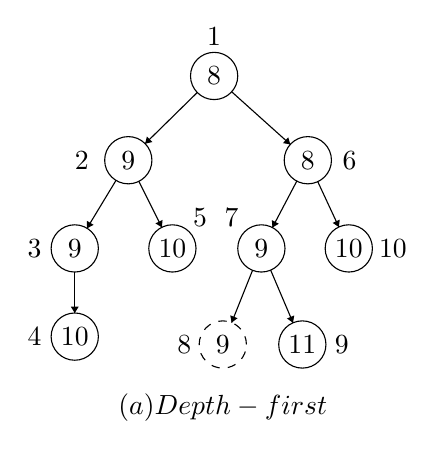
\begin{tikzpicture}[scale=0.1]
				\tikzstyle{every node}+=[inner sep=0pt]
				\draw [black] (34.8,-8) circle (3);
				\draw (34.8,-8) node {$8$};
				\draw (34.8,-3) node {$1$};
				\draw [black] (23.9,-18.7) circle (3);
				\draw (23.9,-18.7) node {$9$};
				\draw (18,-18.7) node {$2$};
				\draw [black] (46.7,-18.7) circle (3);
				\draw (46.7,-18.7) node {$8$};
				\draw (52,-18.7) node {$6$};
				\draw [black] (17.1,-29.9) circle (3);
				\draw (17.1,-29.9) node {$9$};
				\draw (12,-29.9) node {$3$};
				\draw [black] (29.5,-29.9) circle (3);
				\draw (29.5,-29.9) node {$10$};
				\draw (33,-26) node {$5$};
				\draw [black] (17.1,-41.1) circle (3);
				\draw (17.1,-41.1) node {$10$};
				\draw (12,-41.1) node {$4$};
				\draw [black] (40.8,-29.9) circle (3);
				\draw (40.8,-29.9) node {$9$};
				\draw (37,-26) node {$7$};
				\draw [black] (51.9,-29.9) circle (3);
				\draw (51.9,-29.9) node {$10$};
				\draw (57.5,-29.9) node {$10$};
				\draw [dashed] (35.9,-42.1) circle (3);
				\draw (35.9,-42.1) node {$9$};
				\draw (31,-42.1) node {$8$};
				\draw [black] (46,-42.1) circle (3);
				\draw (46,-42.1) node {$11$};
				\draw (51,-42.1) node {$9$};
				\draw [black] (32.66,-10.1) -- (26.04,-16.6);
				\fill [black] (26.04,-16.6) -- (26.96,-16.39) -- (26.26,-15.68);
				\draw [black] (37.03,-10.01) -- (44.47,-16.69);
				\fill [black] (44.47,-16.69) -- (44.21,-15.79) -- (43.54,-16.53);
				\draw [black] (22.34,-21.26) -- (18.66,-27.34);
				\fill [black] (18.66,-27.34) -- (19.5,-26.91) -- (18.64,-26.39);
				\draw [black] (25.24,-21.38) -- (28.16,-27.22);
				\fill [black] (28.16,-27.22) -- (28.25,-26.28) -- (27.35,-26.72);
				\draw [black] (17.1,-32.9) -- (17.1,-38.1);
				\fill [black] (17.1,-38.1) -- (17.6,-37.3) -- (16.6,-37.3);
				\draw [black] (39.68,-32.68) -- (37.02,-39.32);
				\fill [black] (37.02,-39.32) -- (37.78,-38.76) -- (36.85,-38.39);
				\draw [black] (41.98,-32.66) -- (44.82,-39.34);
				\fill [black] (44.82,-39.34) -- (44.97,-38.41) -- (44.05,-38.8);
				\draw [black] (45.3,-21.35) -- (42.2,-27.25);
				\fill [black] (42.2,-27.25) -- (43.01,-26.77) -- (42.13,-26.3);
				\draw [black] (47.96,-21.42) -- (50.64,-27.18);
				\fill [black] (50.64,-27.18) -- (50.75,-26.24) -- (49.85,-26.66);
				\draw (35.9,-50.1) node {$\text{(a) }Depth-first$};
			\end{tikzpicture}\qquad
			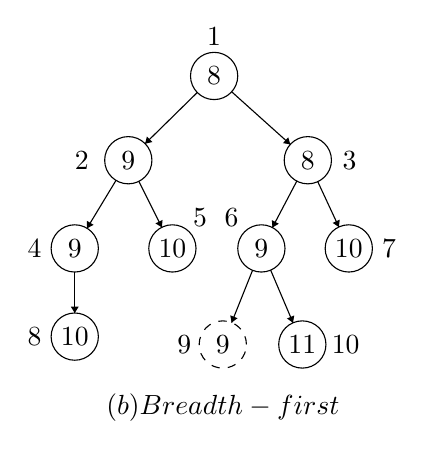
\begin{tikzpicture}[scale=0.1]
				\tikzstyle{every node}+=[inner sep=0pt]
				\draw [black] (34.8,-8) circle (3);
				\draw (34.8,-8) node {$8$};
				\draw (34.8,-3) node {$1$};
				\draw [black] (23.9,-18.7) circle (3);
				\draw (23.9,-18.7) node {$9$};
				\draw (18,-18.7) node {$2$};
				\draw [black] (46.7,-18.7) circle (3);
				\draw (46.7,-18.7) node {$8$};
				\draw (52,-18.7) node {$3$};
				\draw [black] (17.1,-29.9) circle (3);
				\draw (17.1,-29.9) node {$9$};
				\draw (12,-29.9) node {$4$};
				\draw [black] (29.5,-29.9) circle (3);
				\draw (29.5,-29.9) node {$10$};
				\draw (33,-26) node {$5$};
				\draw [black] (17.1,-41.1) circle (3);
				\draw (17.1,-41.1) node {$10$};
				\draw (12,-41.1) node {$8$};
				\draw [black] (40.8,-29.9) circle (3);
				\draw (40.8,-29.9) node {$9$};
				\draw (37,-26) node {$6$};
				\draw [black] (51.9,-29.9) circle (3);
				\draw (51.9,-29.9) node {$10$};
				\draw (57,-29.9) node {$7$};
				\draw [dashed] (35.9,-42.1) circle (3);
				\draw (35.9,-42.1) node {$9$};
				\draw (31,-42.1) node {$9$};
				\draw [black] (46,-42.1) circle (3);
				\draw (46,-42.1) node {$11$};
				\draw (51.5,-42.1) node {$10$};
				\draw [black] (32.66,-10.1) -- (26.04,-16.6);
				\fill [black] (26.04,-16.6) -- (26.96,-16.39) -- (26.26,-15.68);
				\draw [black] (37.03,-10.01) -- (44.47,-16.69);
				\fill [black] (44.47,-16.69) -- (44.21,-15.79) -- (43.54,-16.53);
				\draw [black] (22.34,-21.26) -- (18.66,-27.34);
				\fill [black] (18.66,-27.34) -- (19.5,-26.91) -- (18.64,-26.39);
				\draw [black] (25.24,-21.38) -- (28.16,-27.22);
				\fill [black] (28.16,-27.22) -- (28.25,-26.28) -- (27.35,-26.72);
				\draw [black] (17.1,-32.9) -- (17.1,-38.1);
				\fill [black] (17.1,-38.1) -- (17.6,-37.3) -- (16.6,-37.3);
				\draw [black] (39.68,-32.68) -- (37.02,-39.32);
				\fill [black] (37.02,-39.32) -- (37.78,-38.76) -- (36.85,-38.39);
				\draw [black] (41.98,-32.66) -- (44.82,-39.34);
				\fill [black] (44.82,-39.34) -- (44.97,-38.41) -- (44.05,-38.8);
				\draw [black] (45.3,-21.35) -- (42.2,-27.25);
				\fill [black] (42.2,-27.25) -- (43.01,-26.77) -- (42.13,-26.3);
				\draw [black] (47.96,-21.42) -- (50.64,-27.18);
				\fill [black] (50.64,-27.18) -- (50.75,-26.24) -- (49.85,-26.66);
				\draw (35.9,-50.1) node {$\text{(b) }Breadth-first$};
			\end{tikzpicture}\qquad
			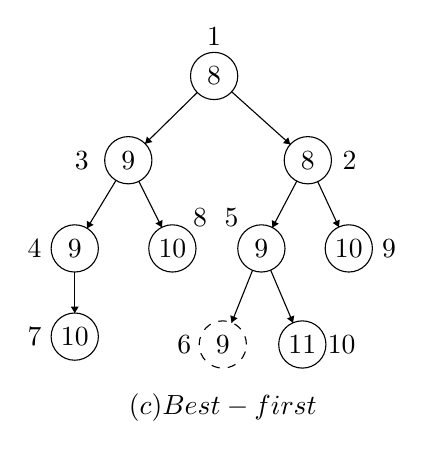
\begin{tikzpicture}[scale=0.1]
				\tikzstyle{every node}+=[inner sep=0pt]
				\draw [black] (34.8,-8) circle (3);
				\draw (34.8,-8) node {$8$};
				\draw (34.8,-3) node {$1$};
				\draw [black] (23.9,-18.7) circle (3);
				\draw (23.9,-18.7) node {$9$};
				\draw (18,-18.7) node {$3$};
				\draw [black] (46.7,-18.7) circle (3);
				\draw (46.7,-18.7) node {$8$};
				\draw (52,-18.7) node {$2$};
				\draw [black] (17.1,-29.9) circle (3);
				\draw (17.1,-29.9) node {$9$};
				\draw (12,-29.9) node {$4$};
				\draw [black] (29.5,-29.9) circle (3);
				\draw (29.5,-29.9) node {$10$};
				\draw (33,-26) node {$8$};
				\draw [black] (17.1,-41.1) circle (3);
				\draw (17.1,-41.1) node {$10$};
				\draw (12,-41.1) node {$7$};
				\draw [black] (40.8,-29.9) circle (3);
				\draw (40.8,-29.9) node {$9$};
				\draw (37,-26) node {$5$};
				\draw [black] (51.9,-29.9) circle (3);
				\draw (51.9,-29.9) node {$10$};
				\draw (57,-29.9) node {$9$};
				\draw [dashed] (35.9,-42.1) circle (3);
				\draw (35.9,-42.1) node {$9$};
				\draw (31,-42.1) node {$6$};
				\draw [black] (46,-42.1) circle (3);
				\draw (46,-42.1) node {$11$};
				\draw (51,-42.1) node {$10$};
				\draw [black] (32.66,-10.1) -- (26.04,-16.6);
				\fill [black] (26.04,-16.6) -- (26.96,-16.39) -- (26.26,-15.68);
				\draw [black] (37.03,-10.01) -- (44.47,-16.69);
				\fill [black] (44.47,-16.69) -- (44.21,-15.79) -- (43.54,-16.53);
				\draw [black] (22.34,-21.26) -- (18.66,-27.34);
				\fill [black] (18.66,-27.34) -- (19.5,-26.91) -- (18.64,-26.39);
				\draw [black] (25.24,-21.38) -- (28.16,-27.22);
				\fill [black] (28.16,-27.22) -- (28.25,-26.28) -- (27.35,-26.72);
				\draw [black] (17.1,-32.9) -- (17.1,-38.1);
				\fill [black] (17.1,-38.1) -- (17.6,-37.3) -- (16.6,-37.3);
				\draw [black] (39.68,-32.68) -- (37.02,-39.32);
				\fill [black] (37.02,-39.32) -- (37.78,-38.76) -- (36.85,-38.39);
				\draw [black] (41.98,-32.66) -- (44.82,-39.34);
				\fill [black] (44.82,-39.34) -- (44.97,-38.41) -- (44.05,-38.8);
				\draw [black] (45.3,-21.35) -- (42.2,-27.25);
				\fill [black] (42.2,-27.25) -- (43.01,-26.77) -- (42.13,-26.3);
				\draw [black] (47.96,-21.42) -- (50.64,-27.18);
				\fill [black] (50.64,-27.18) -- (50.75,-26.24) -- (49.85,-26.66);
				\draw (35.9,-50.1) node {$\text{(c) } Best-first$};
			\end{tikzpicture}\qquad
		\end{center}
		\caption{\doublespacing Sub-tree traversals for different searching techniques. The numbers on the side of each node correspond to the lower-bound at that step and the dotted node represents the optimal solution \cite{morrison2016branch}.}
		\label{fig:searchTechniques}
	\end{figure}
		\subsubsection{Depth-First}
			The depth-first search strategy follows a last-in, first-out order and is implemented by maintaining a list of unexplored nodes in a stack as shown in Figure \ref{fig:searchTechniques} (a). 
			The routine removes the top element from the stack to explore for the next sub-problem and the children generated are inserted on the top of the stack. The potential memory requirements needed to maintain a list of children nodes can become a problem, however we remedy this by maintaining a path of indices from the root to the current node instead of the entire list of unexplored sub-problems.
			When the current sub-problem is complete, the algorithm selects the next unexplored node for exploration and if one does not exist, the algorithm backtracks to the nearest ancestor node. 
			The biggest issue with this technique is that it is blind to the structure of the problem and makes no use of the lower bounds encountered during a traversal. 
			This can cause the algorithm to spend large amounts of time exploring unpromising regions, especially when the search space is unbalanced. 
			This results in a running time of $\Theta (V+E)$ \cite{cormen2009introduction}, however DFS yields valuable information about the structure of a graph.
		\subsubsection{Breadth-First}
			The breadth-first search strategy, shown in Figure \ref{fig:searchTechniques} (b), explores nodes based on a first-in, first-out order and is implemented by maintaining a queue data structure. 
			This results in the algorithm exploring all nodes at the same level before moving on to deeper portions of the tree. 
			The advantage of this technique is that if the optimal solution is close to the root, or the tree is unbalanced, breadth-first search will find the solution faster than depth-first. 
			However, if the solution occurs at lower depths, breadth-first can require large amounts of memory because it does not take advantage of any pruning rules. 
			The BFS technique runs on a running time of $O(V+E)$ \cite{cormen2009introduction} and is linear to the size of an adjacency list representation of the graph.
		\subsubsection{Best-First}
			The best-first search strategy is often used when memory considerations are of no concern. This technique stores the entire unexplored search space and applies a heuristic function to every unexplored node and selects the node that returns the minimum value. 
			We say that the heuristic function is admissible if it never overestimates the best solution and is often referred to as the $A^*$  method. The technique is implemented as a heap data structure and the order of a traversal can be seen in Figure \ref{fig:searchTechniques} (c). 
			The complexity of $A^*$ depends on the heuristic used.
			In an unbounded search space, the worst case running time can reach $O(b^d)$ \cite{russell2010artificial} where $d$ is the shortest path to a solution and $b$ is the branching factor. 
		%! Author = rickr
%! Date = 11/17/2021

\subsection{Pruning Rules}
	The pruning rules of Algorithm \ref{alg: pseudocode} determine whether or not $S$ can be fathomed.
	While the use of a heuristic allows us to approximate the utility of a state without performing a complete search, pruning rules allow us to neglect portions of the tree without affecting the final choice. 
	Many of the pruning techniques are developed in the context of Artificial Intelligence, however the basic function holds across all applications involving combinatorial optimization. 
	\subsubsection{Lower-Bound}
		Producing a lower bound on the objective function at each node is the most common way to prune a search space \cite{morrison2016branch}. 
		The lower bound then used to prune sub-problems who's lower bound is no better than the incumbent solution. 
		The value of the lower bound is calculated by relaxing aspects of the problem, and as such, some lower bound calculations may be easier to determine than others. 
		The general technique is to attempt pruning with a lower bound that is easy to calculate before moving on to more complex (but possibly tighter) lower bounds. 
	\subsubsection{Alpha-Beta Pruning}
		Alpha-beta pruning is often used in areas of artificial intelligence that employ a MinMax decision rule for minimizing the possible loss of a worst case scenario. 
		The idea is to maximize the minimum gain, however, issues arise when the number of game states to examine is exponential in the depth of the tree. 
		Alpha-beta pruning, while not eliminating the exponent, effectively cuts it in half by assigning a numerical score to each terminal node \cite{russell2010artificial}. 
		Each terminal node represents the outcome of the player with the next move.
		The technique is referred to as an adversarial search algorithm because the game tree can represent many two-player zero-sum games. 
		Two values $\alpha$ and $\beta$ represent the minimum score that the maximizing player is assured of, and maximum score that the minimizing player is assured of. 
		When the value of a terminal node results in $\beta$ being less than $\alpha$, the maximizing player may ignore descendants of the node.  
	\subsubsection{Decision Tree Pruning}
		For some problems, it is found that decision-tree learning algorithms can generate large trees with no inherent pattern. This can happen when too many irrelevant features are fed into the training model. 
		For example, when measuring the outcome of a tossed coin, the color, time of day, the exact person doing the flipping, have no effect on the outcome. 
		However, if the model is provided these features as input, then the training could be subject to over-fitting. 
		In general, over-fitting is more likely to occur when the hypothesis space and number of input attributes grows \cite{russell2010artificial}. 
		To combat this, we use decision-tree pruning. 
		The general idea is that we start with a full tree and look at a test node whose descendants are only leaf nodes. 
		If testing detects only noise in the data, then we eliminate the node and replace it with the leaf node. 
	
		%! Author = rickr
%! Date = 11/27/2021
\subsection{Branching Strategies}
	The branching strategy affects the number of children and the way the sub-problems generated in Algorithm \ref{alg: pseudocode} are partitioned. 